\chapter{Конструкторский раздел}



\section{Основные концепции менеджера памяти}

В общем случае, эффективность менеджера памяти определяется следующими факторами:

\begin{enumerate}[label*=\arabic*.]
	\item \textbf{Задержка мутатора при выполнении операций выделения памяти и получения доступа к объектам.} При выполнении этих операций основная программа блокируется в ожидании обслуживания запроса к менеджеру памяти. Поэтому одной из его задач является минимизация времени блокировки мутатора.
	\item \textbf{Доля процессорного времени, затрачиваемая на сбор мусора.} Если сборщик мусора работает конкурентно с основной программой, то он отнимает процессорное время, выделенное программе операционной системой. Задачей сборщика является избежание ситуаций, при которых частая сборка мусора приводит к перегрузкам, замедляющим основную программу.
	\item \textbf{Накладные расходы памяти на хранение данных об обрабатываемых объектах.} Их минимизация повышает эффективность выделения памяти, однако, возможно, в ущерб трудоёмкости алгоритма сборки мусора.
	\item \textbf{Использование конкурентной сборки мусора.} Для снижения среднего времени паузы мутатора сборщик мусора может выполнять её конкурентно с потоками основной программы.
	\item \textbf{Использование параллельной сборки мусора.} Задействование сборщиком сразу нескольких потоков программы может ускорить его работу.
	\item \textbf{Использование алгоритма поколений.} Следование гипотезе поколений (см. п. \ref{generations}) позволяет снизить время одного цикла сборки мусора без потери её эффективности. Эффективность цикла сборки мусора можно оценить объёмом памяти, освобождённым за единицу времени.
\end{enumerate}

Целью разрабатываемого метода распределения памяти является минимизация нагрузки на мутатор за счёт использование параллельной и конкурентной сборки мусора.

Для организации объектов, обрабатываемых менеджером памяти, предлагается использовать модель поколений (см. п. \ref{generations}), предполагающей наличие молодого, промежуточного и старого поколения. Промежуточное поколение необходимо для того, чтобы замедлить продвижение объектов по поколениям. Если объект пережил один сбор мусора, то это не значит, что он будет жить дольше других объектов. А вот если он пережил два сбора мусора, то есть его возраст больше промежутка времени между сборами мусора, то вероятность его дальнейшего выживания оценивается выше.

Для реализации модели поколений куча разделяется на три пространства (поколения). Каждый новый объект помещается в первое поколение. Алгоритм сбора мусора выполняется только над объектами определённых поколений, и если объект не уничтожается во время обработки своего поколения, он будет перемещён в следующее поколение, где его будут анализировать реже. Если тот же объект не уничтожается после ещё одного цикла сборки мусора, он будет перемещен в последнее поколение, где его будут анализировать реже всего. Первоначально сборка мусора выполняется только в первом поколении. Такой подход позволяет сборщику мусора избежать сканирования всей кучи на каждом цикле сборки за счёт их разбиения на более короткие. В таком случае сборщик будет выполнять свою работу инкрементально, с каждым новым циклом увеличивая количество обрабатываемых объектов и охватывая более старые объекты.

Для контроля фрагментации кучи предлагается разделить пространство каждого поколения на \textbf{арены памяти} фиксированного размера, определяемого особенностями языка реализации. Предполагается, что именно арена будет являться единицей перераспределения памяти между поколениями. Это означает, что после циклов сборки мусора объекты будут перемещаться между аренами не по одному, а множеством. Такой подход позволит в некоторой степени сохранить эффективное расположение ссылок (см. п. \ref{reference_locality}).



\section{Проектирование алгоритмов распределения памяти}

\subsection{Представление дескриптора объекта}

Для управления объектами программы разрабатываемый менеджер памяти должен хранить следующие данные о них:

\begin{itemize}[label*=---]
	\item адрес для обеспечения доступа к объекту;
	\item метаданные о типе объекта для анализа его ссылок на другие объекты программы;
	\item арена памяти, в которой был выделен объект, для анализа загруженности арен;
	\item число ссылок на объект;
	\item данные о том, были ли финализированы все ссылки на объект;
	\item данные о том, участвует ли объект в цикле ссылок;
	\item идентификатор последнего цикла сборки мусора, в котором участвовал объект, для определения того, был ли размечен объект на текущем цикле сборки.
\end{itemize}

Также для избежания гонок данных при работе с дескриптором объекта он должен содержать примитив блокировки для осуществления атомарных операций над ним.

Для определения, является ли объект мусором, предлагается проверять следующие условия:

\begin{enumerate}[label*=\arabic*)]
	\item все ссылки на объект были финализированы;
	\item объект участвует в цикле ссылок и количество ссылок на него не превышает 1.
\end{enumerate}

Условие 1 не является достаточным для определения недостижимости объекта в основной программе, поскольку он может участвовать в цикле ссылок между мусорными объектами. В таком случае предлагается использование дизъюнкции условий 1 и 2 для определения достижимости объекта. Условие 1 соответствует состоянию счётчика ссылок на объект, а условие 2 предполагает осуществление трассирующей сборки мусора для определения циклических ссылок между объектами программы.

Стоит отметить, что ограничение по количеству ссылок на объект в условии 2 не даёт возможность идентифицировать мусорными те объекты, которые участвуют одновременно в нескольких циклах ссылок. Это означает, что сборщик мусора не сможет за один цикл сборки освободить все объекты, участвующие в пересекающихся циклах ссылок, опираясь на предположение о том, что подобные случаи будут встречаться в программах относительно редко. К тому же, для корректной идентификации объектов, участвующих в нескольких циклах ссылок, пришлось бы использовать алгоритмы обнаружения компонент сильной связности в орграфах, которые образуют объекты с помощью отношения ссылки. Примерами таких алгоритмов могут послужить алгоритмы Тарьяна и Косарайю \cite{graph_algorithms}. Их использование может существенно увеличить трудоёмкость алгоритмов сборки мусора.

\subsection{Алгоритм выделения памяти}

На рисунке \ref{fig:allocation} представлен алгоритм выделения памяти.

\begin{figure}[H]
	\centering
	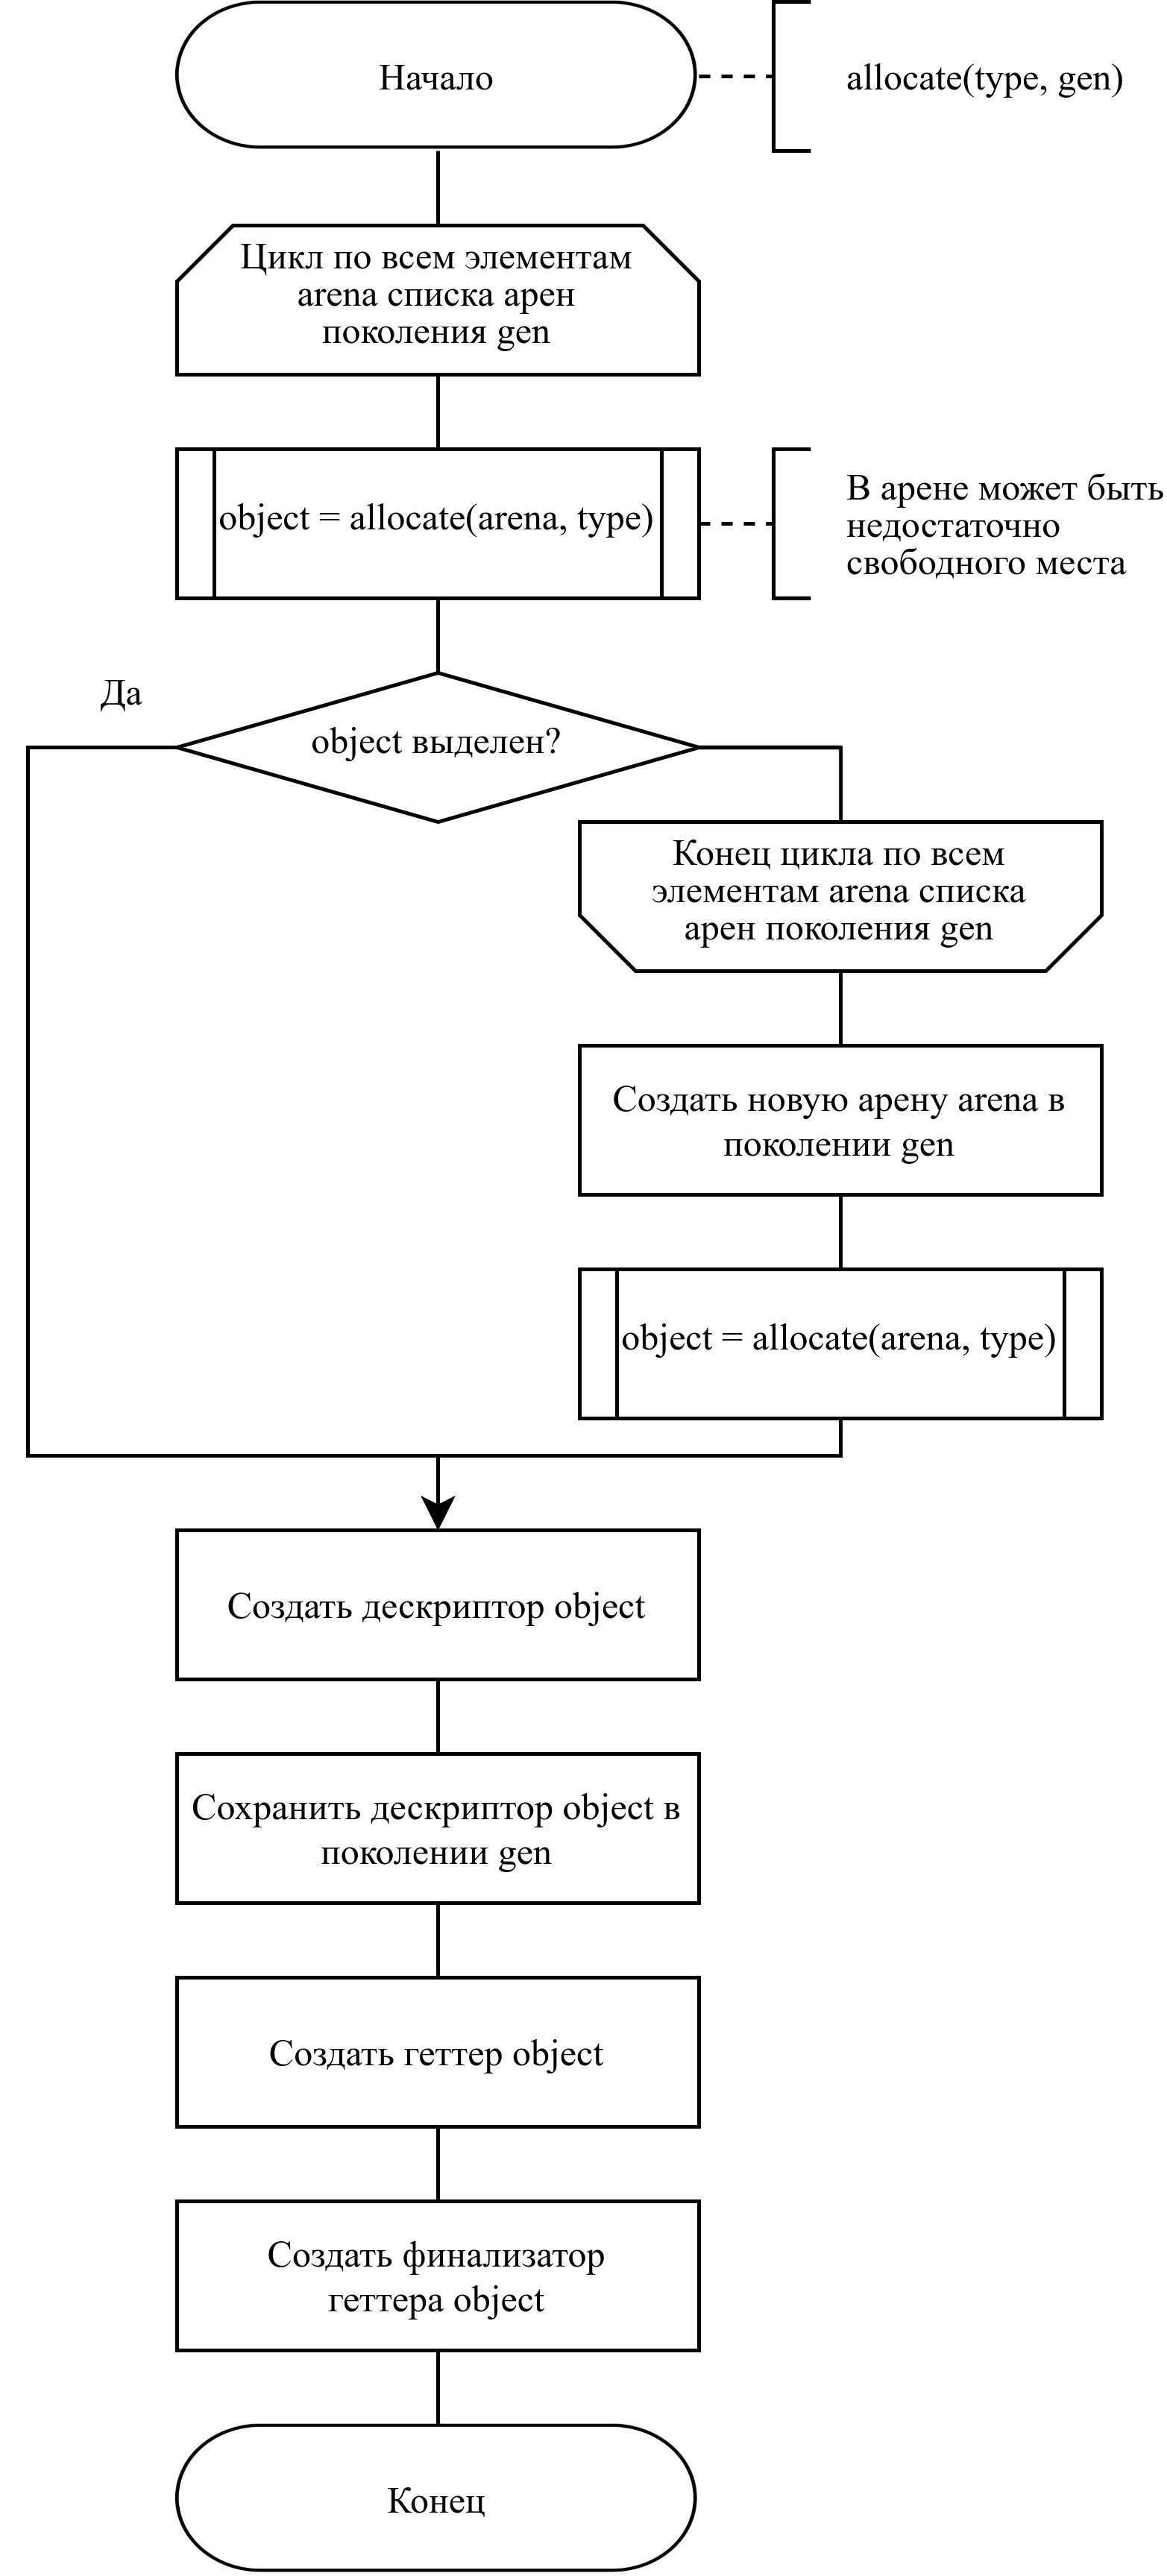
\includegraphics[scale=0.19]{assets/allocate.png}
	\caption{Алгоритм выделения памяти}
	\label{fig:allocation}
\end{figure}

Предполагается, что геттер объекта будет использоваться мутатором как ссылка на него, поскольку геттер предоставляет единственный вариант получения доступа к объекту из основной программы. Геттер является барьером между основной программой и менеджером памяти, предотвращающим гонки данных между ними.

АССИМПТОТИЧЕСКАЯ ОЦЕНКА СЛОЖНОСТИ АЛГОРИТМОВ ДЛЯ ОПРЕДЕЛЕНИЯ ГАРАНТИИ ВРЕМЕНИ ИСПОЛНЕНИЯ?????

% Гарантия времени выполнения разрабатываемого метода подразумевает ограничение времени, которое пользовательская программа затрачивает на вызовы реализации метода, то есть на выделение памяти и обращение к выделенным объектам. Время выполнения обращения к объекту 

% Дать асимптотическую оценку временной сложности алгоритма выделения

\subsection{Алгоритм сбора циклических ссылок}

Для сбора циклических ссылок между объектами программы предлагается использование трассирующей сборки мусора.

Каждая следующая сборка мусора выполняется после того, как был выделен дополнительный объём памяти, пропорциональный тому, который был зафиксирован при предыдущем запуске сборки мусора. Данная пропорция должна конфигурироваться с помощью переменной среды выполнения программы, чтобы пользователь мог настраивать частоту сборки мусора. Например, если переменная среды равна 100 и программа использует 4 Мб памяти, следующий цикл сборки мусора запустится только тогда, когда объём используемой памяти достигнет 8 Мб. Такая настройка позволяет сохранить линейную зависимость накладных расходов на сборку мусора от накладных расходов на выделение памяти. Переменная среды просто изменяет линейную константу.

Также сам пользователь должен иметь возможность явно вызывать сборку мусора. Это может понадобиться для того, чтобы предотвратить сбор мусора в критический период, например, при большой нагрузке на сервер. В таком случае пользователь может определить момент, когда сервер не обрабатывает запросы, и вызвать сборку мусора.

Сбор мусора предлагается осуществлять по алгоритму \textbf{mark-sweep} (см. п. \ref{tracing}), который не предполагает уплотнения кучи. Такой подход позволяет избежать накладных расходов на копирование объектов, жертвуя их непрерывным последовательным распределением.

Сбор циклических ссылок будет выполняться в три фазы: разметка, очистка и перераспределение объектов между поколениями.

\subsubsection{Разметка}

На рисунке \ref{fig:mark-1} представлен алгоритм разметки объектов нового поколения. Для ускорения разметки предлагается выполнять её в нескольких потоках программы. Параллелизм может быть ограничен путём использования пула потоков. Стоит заметить, что перед началом разметки в счётчике ссылок каждого объекта устанавливается значение -1, так как каждый объект будет обработан не менее одного раза, независимо от того, есть на него ссылки или нет.

\begin{figure}[H]
	\centering
	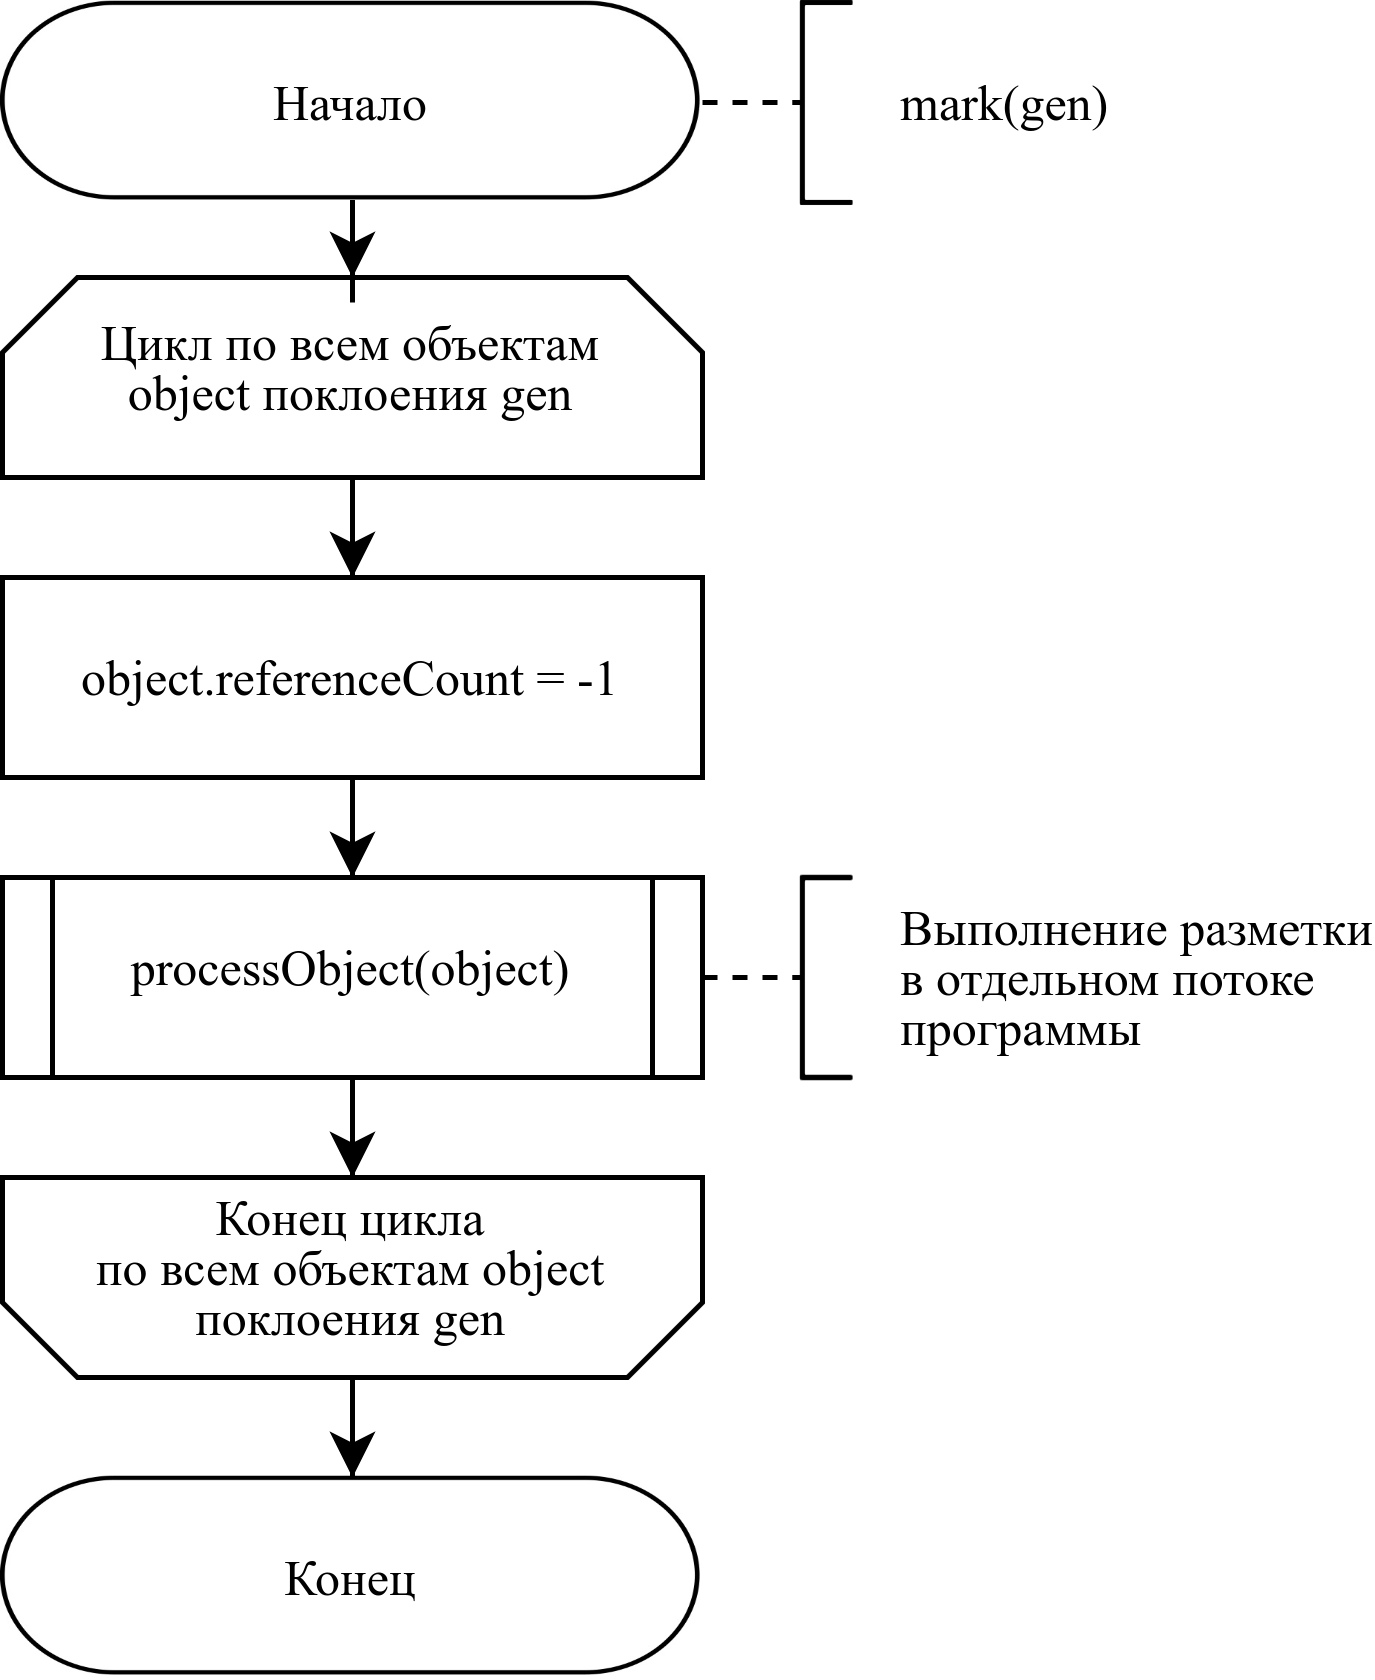
\includegraphics[scale=0.185]{assets/mark-1.png}
	\caption{Алгоритм разметки объектов поколения}
	\label{fig:mark-1}
\end{figure}

На рисунке \ref{fig:mark-2} представлен алгоритм обработки одного объекта, включающий в себя его разметку и анализ ссылок на другие объекты программы, если данный объект ранее не был проанализирован. Также анализ объекта может быть пропущен, если были финализированы все ссылки на него. Выполнение этого условия гарантирует, что рассматриваемый объект является мусором.

\begin{figure}[H]
	\centering
	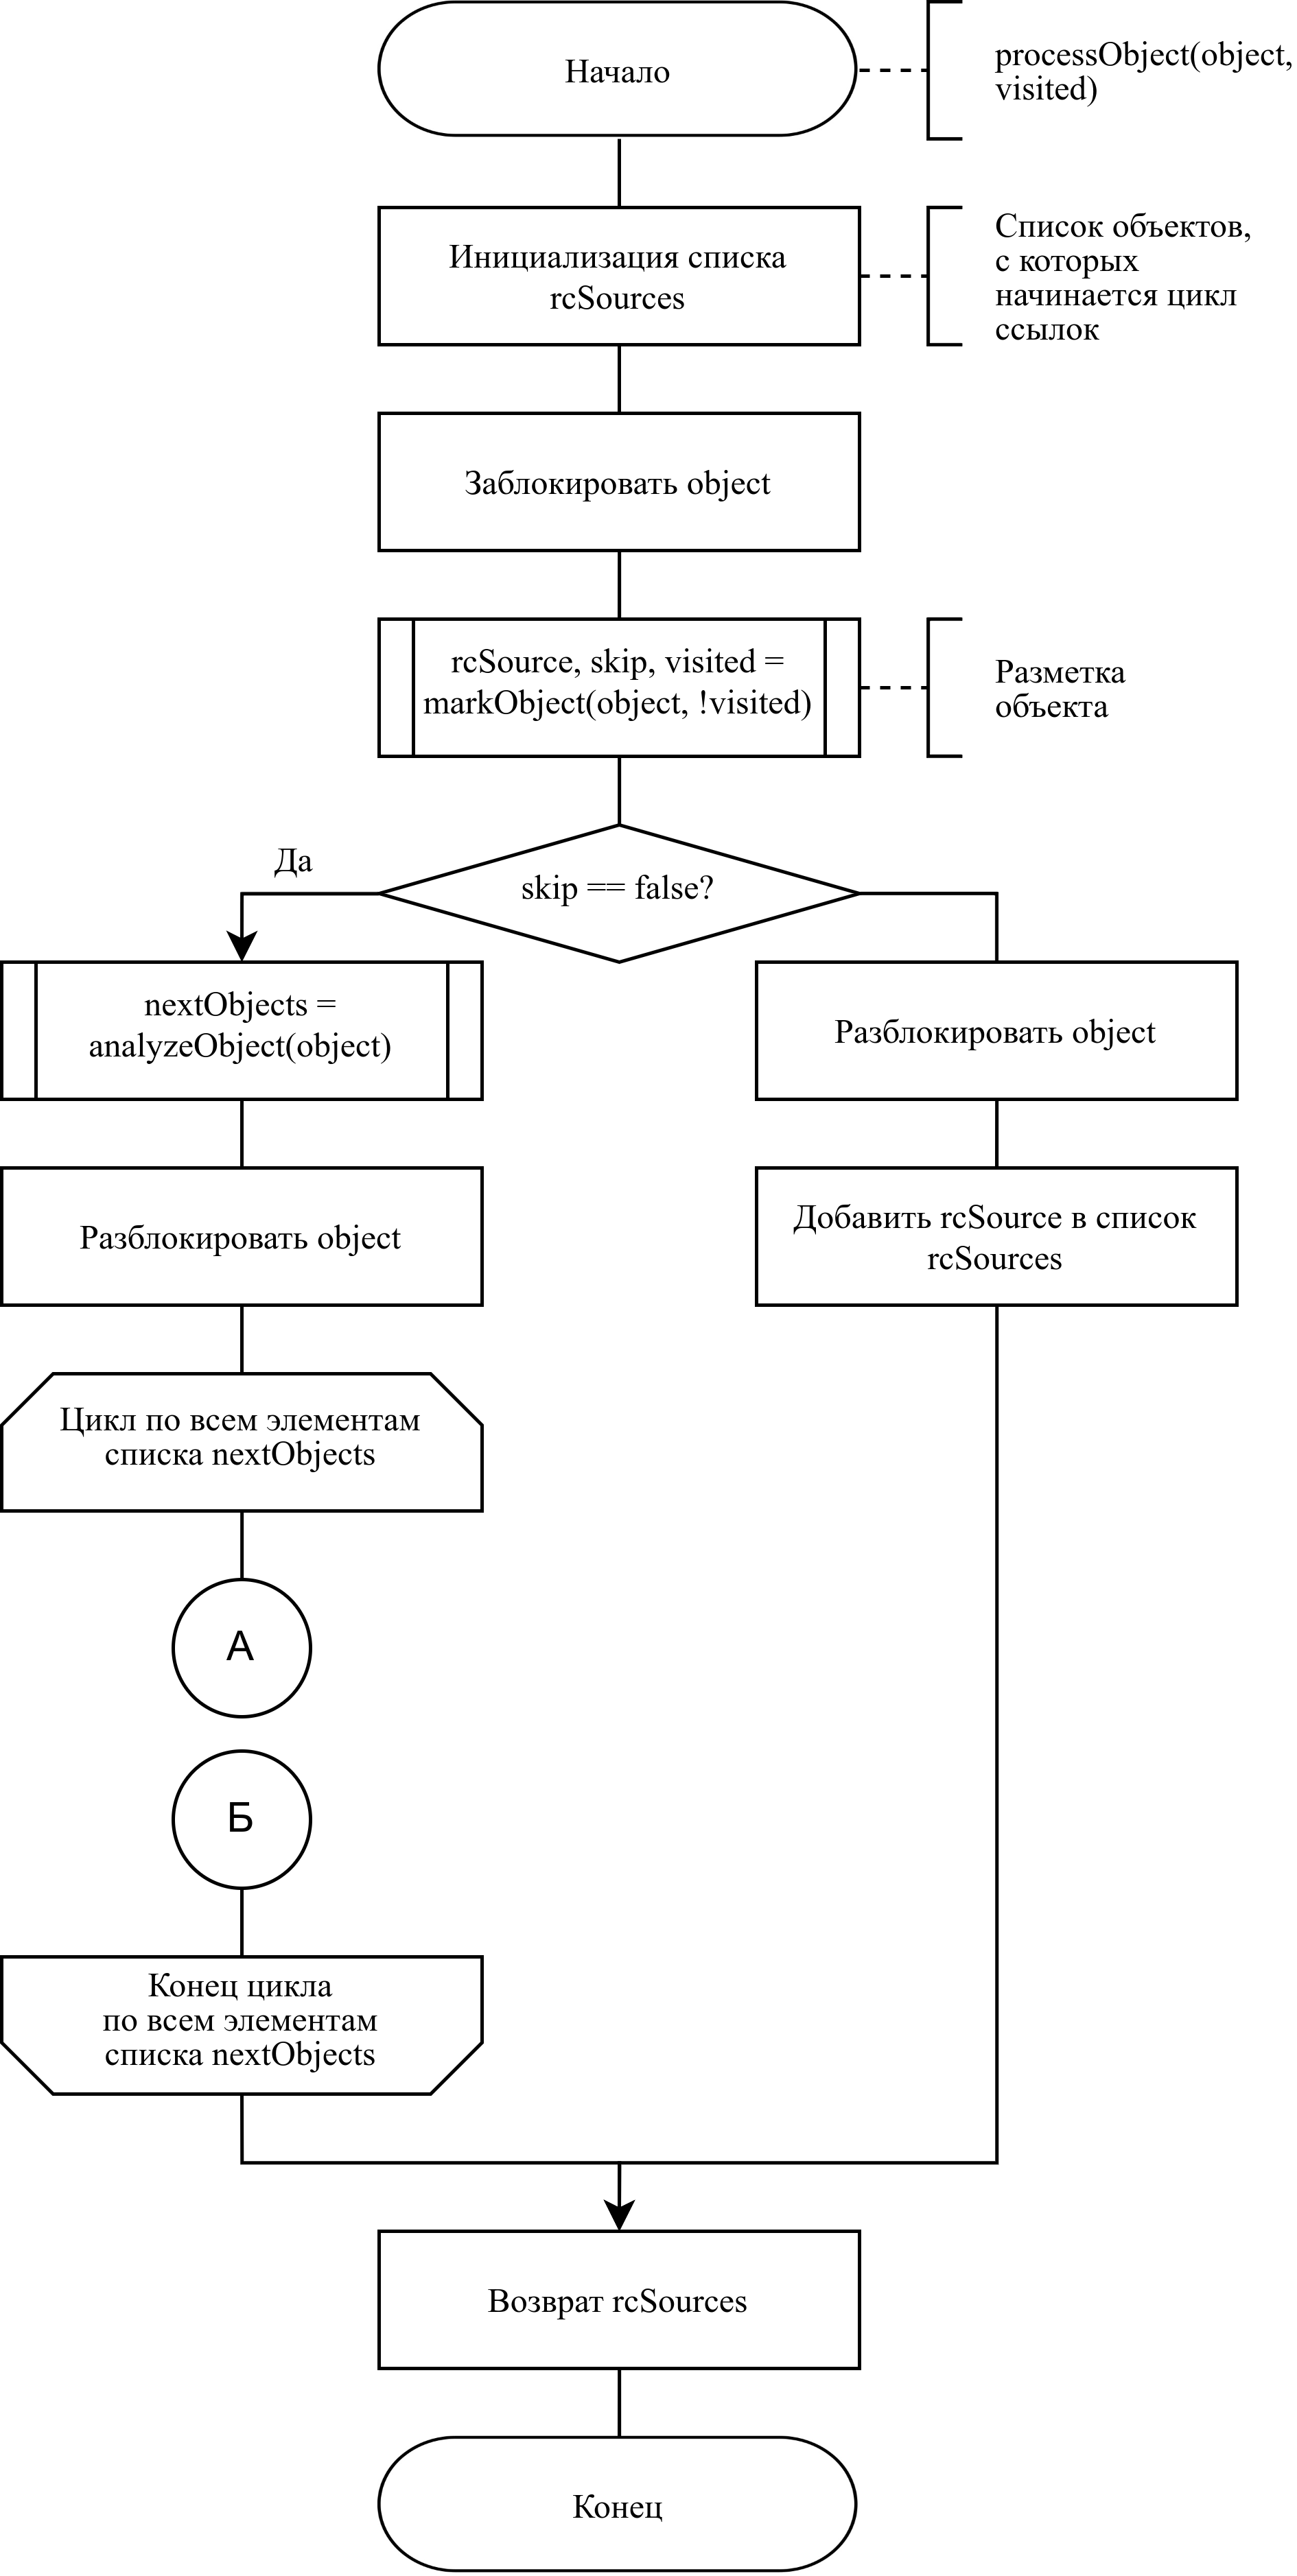
\includegraphics[scale=0.185]{assets/mark-2.png}
	\caption{Алгоритм обработки одного объекта}
	\label{fig:mark-2}
\end{figure}

На рисунке \ref{fig:mark-3} представлен алгоритм разметки объекта, цель которого состоит в том, чтобы заполнить или актуализировать его дескриптор, а также сделать вывод о том, следует ли анализировать его ссылки на другие объекты.

\begin{figure}[H]
	\centering
	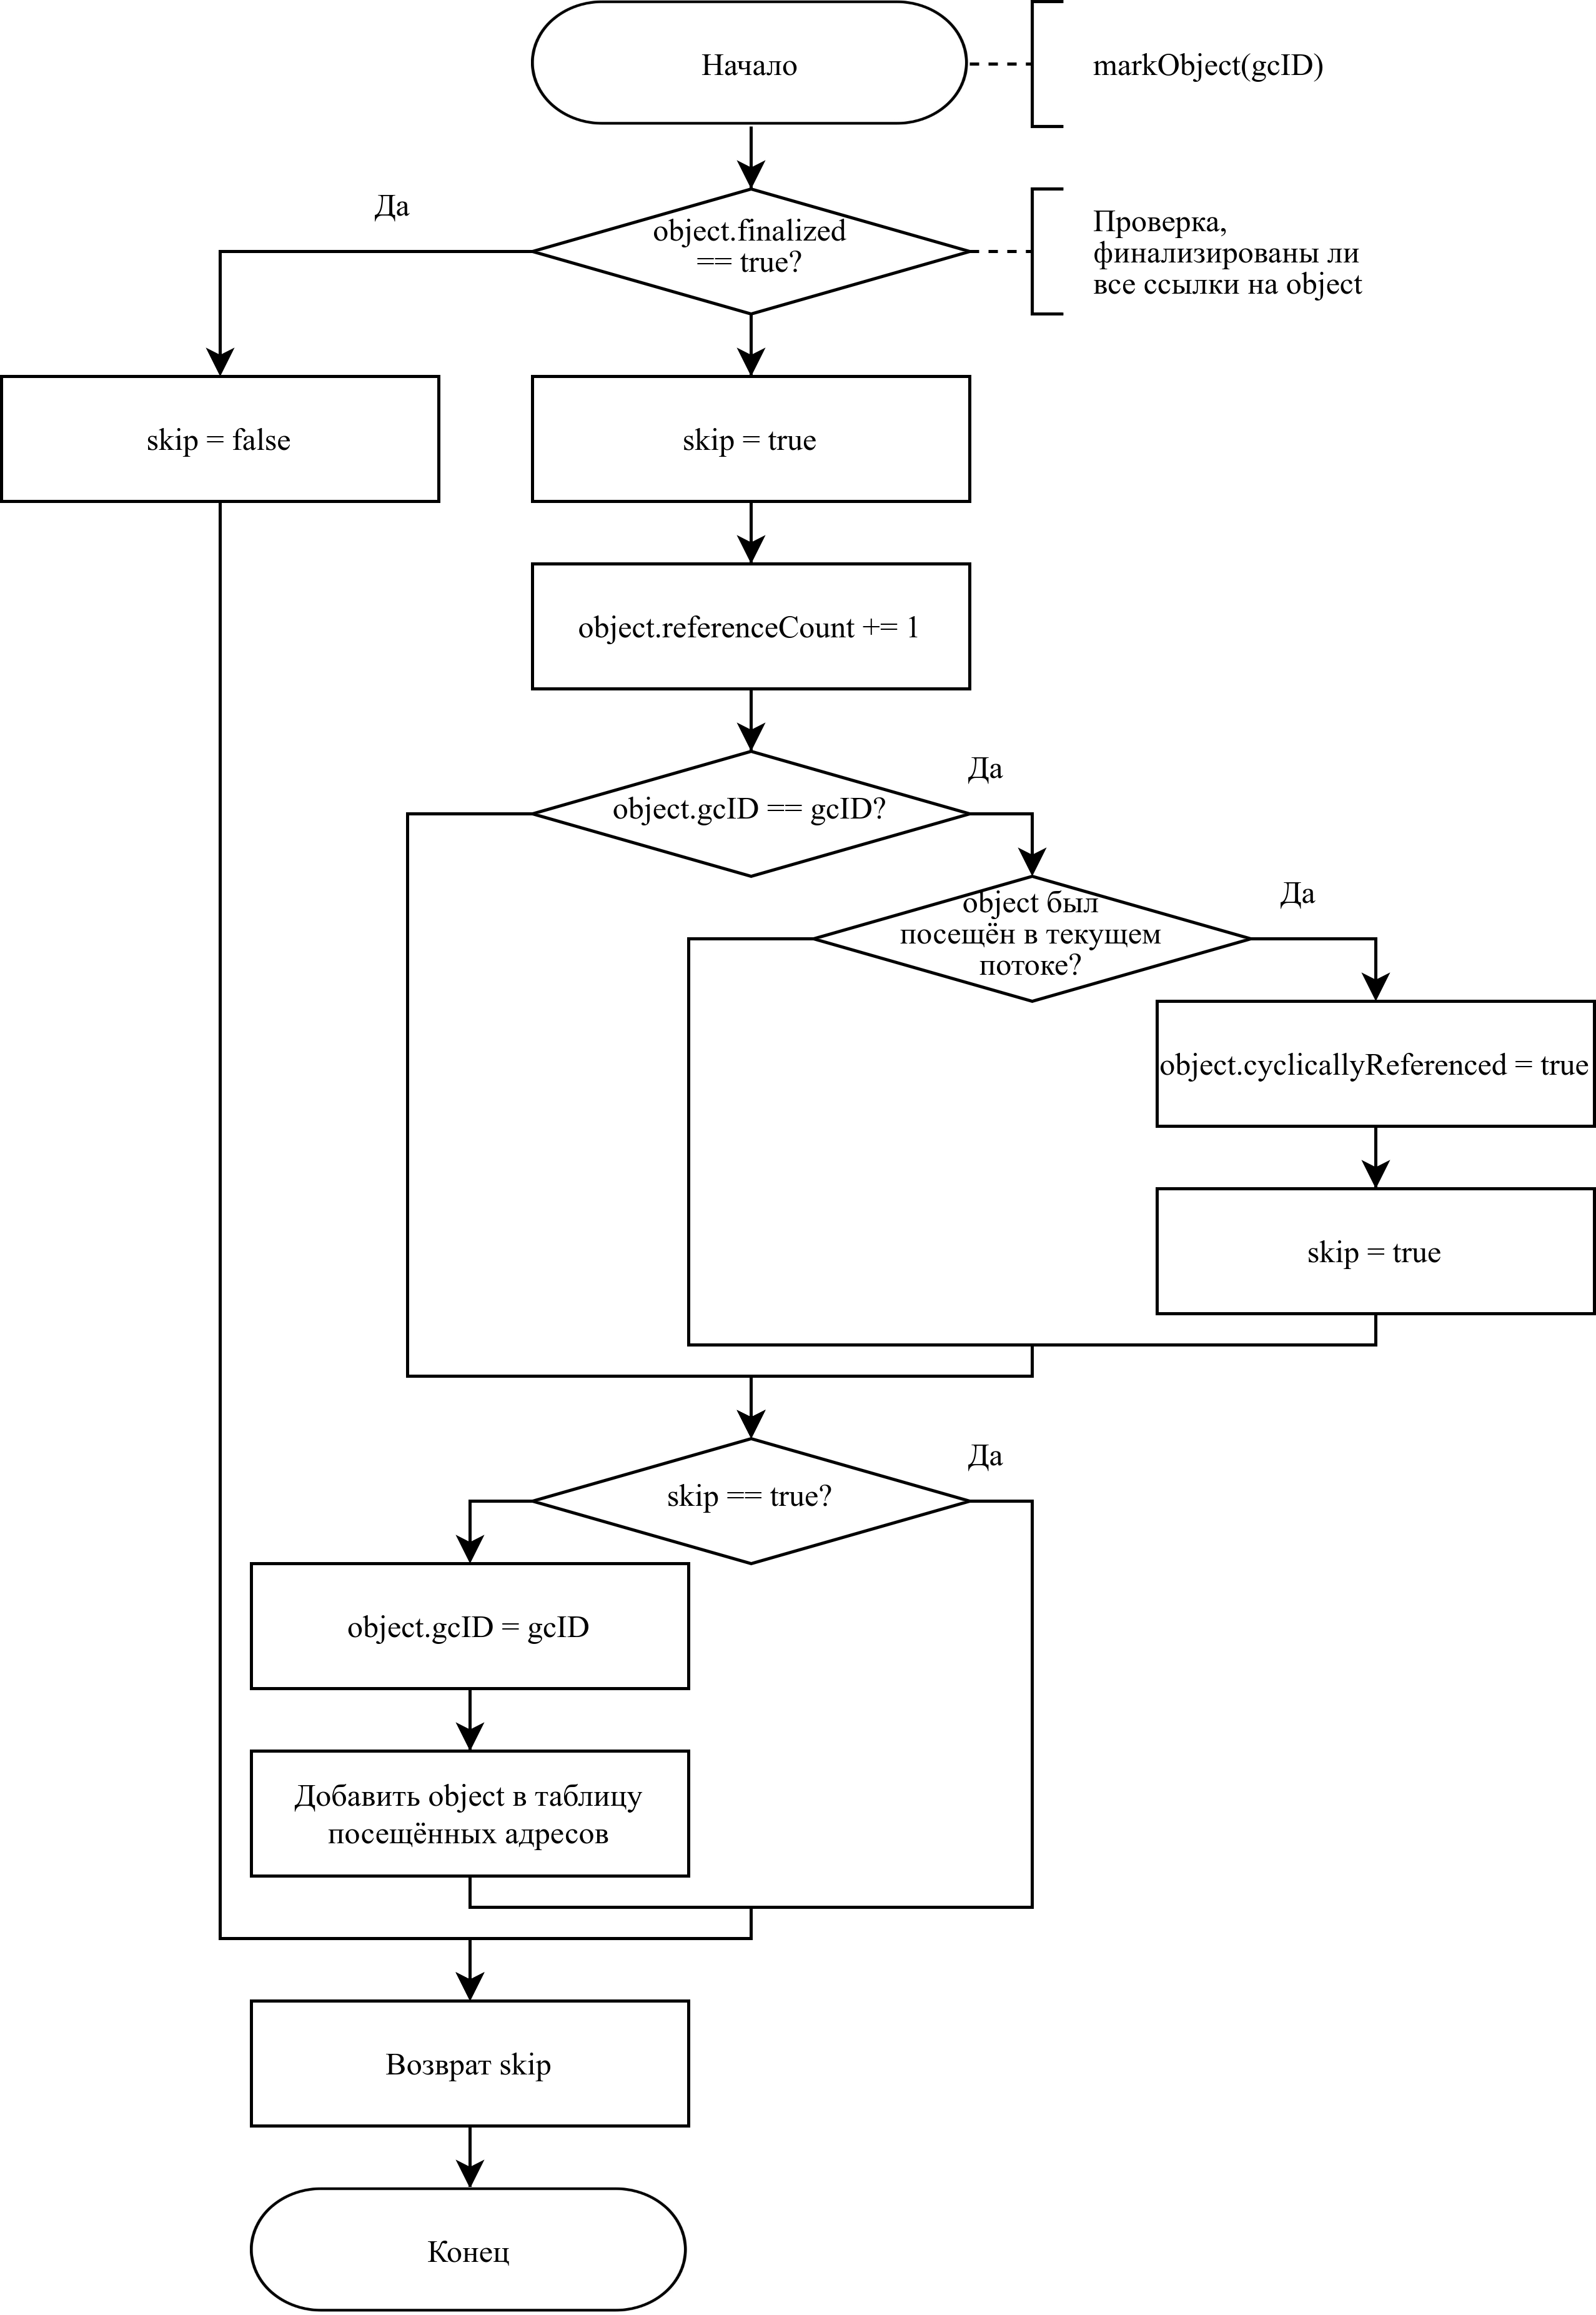
\includegraphics[scale=0.185]{assets/mark-3.png}
	\caption{Алгоритм разметки объекта}
	\label{fig:mark-3}
\end{figure}

На рисунке \ref{fig:mark-4} представлен алгоритм анализа ссылок объекта на другие объекты программы. Ссылка на объект анализируется только в том случае, если она принадлежит множеству объектов, анализируемых на данном цикле сборки мусора. С каждым последующим циклом сбора данное множество расширяется за счёт совокупного анализа всё большего количества поколений, обеспечивая инкрементальное выполнение сборки мусора.

\begin{figure}[H]
	\centering
	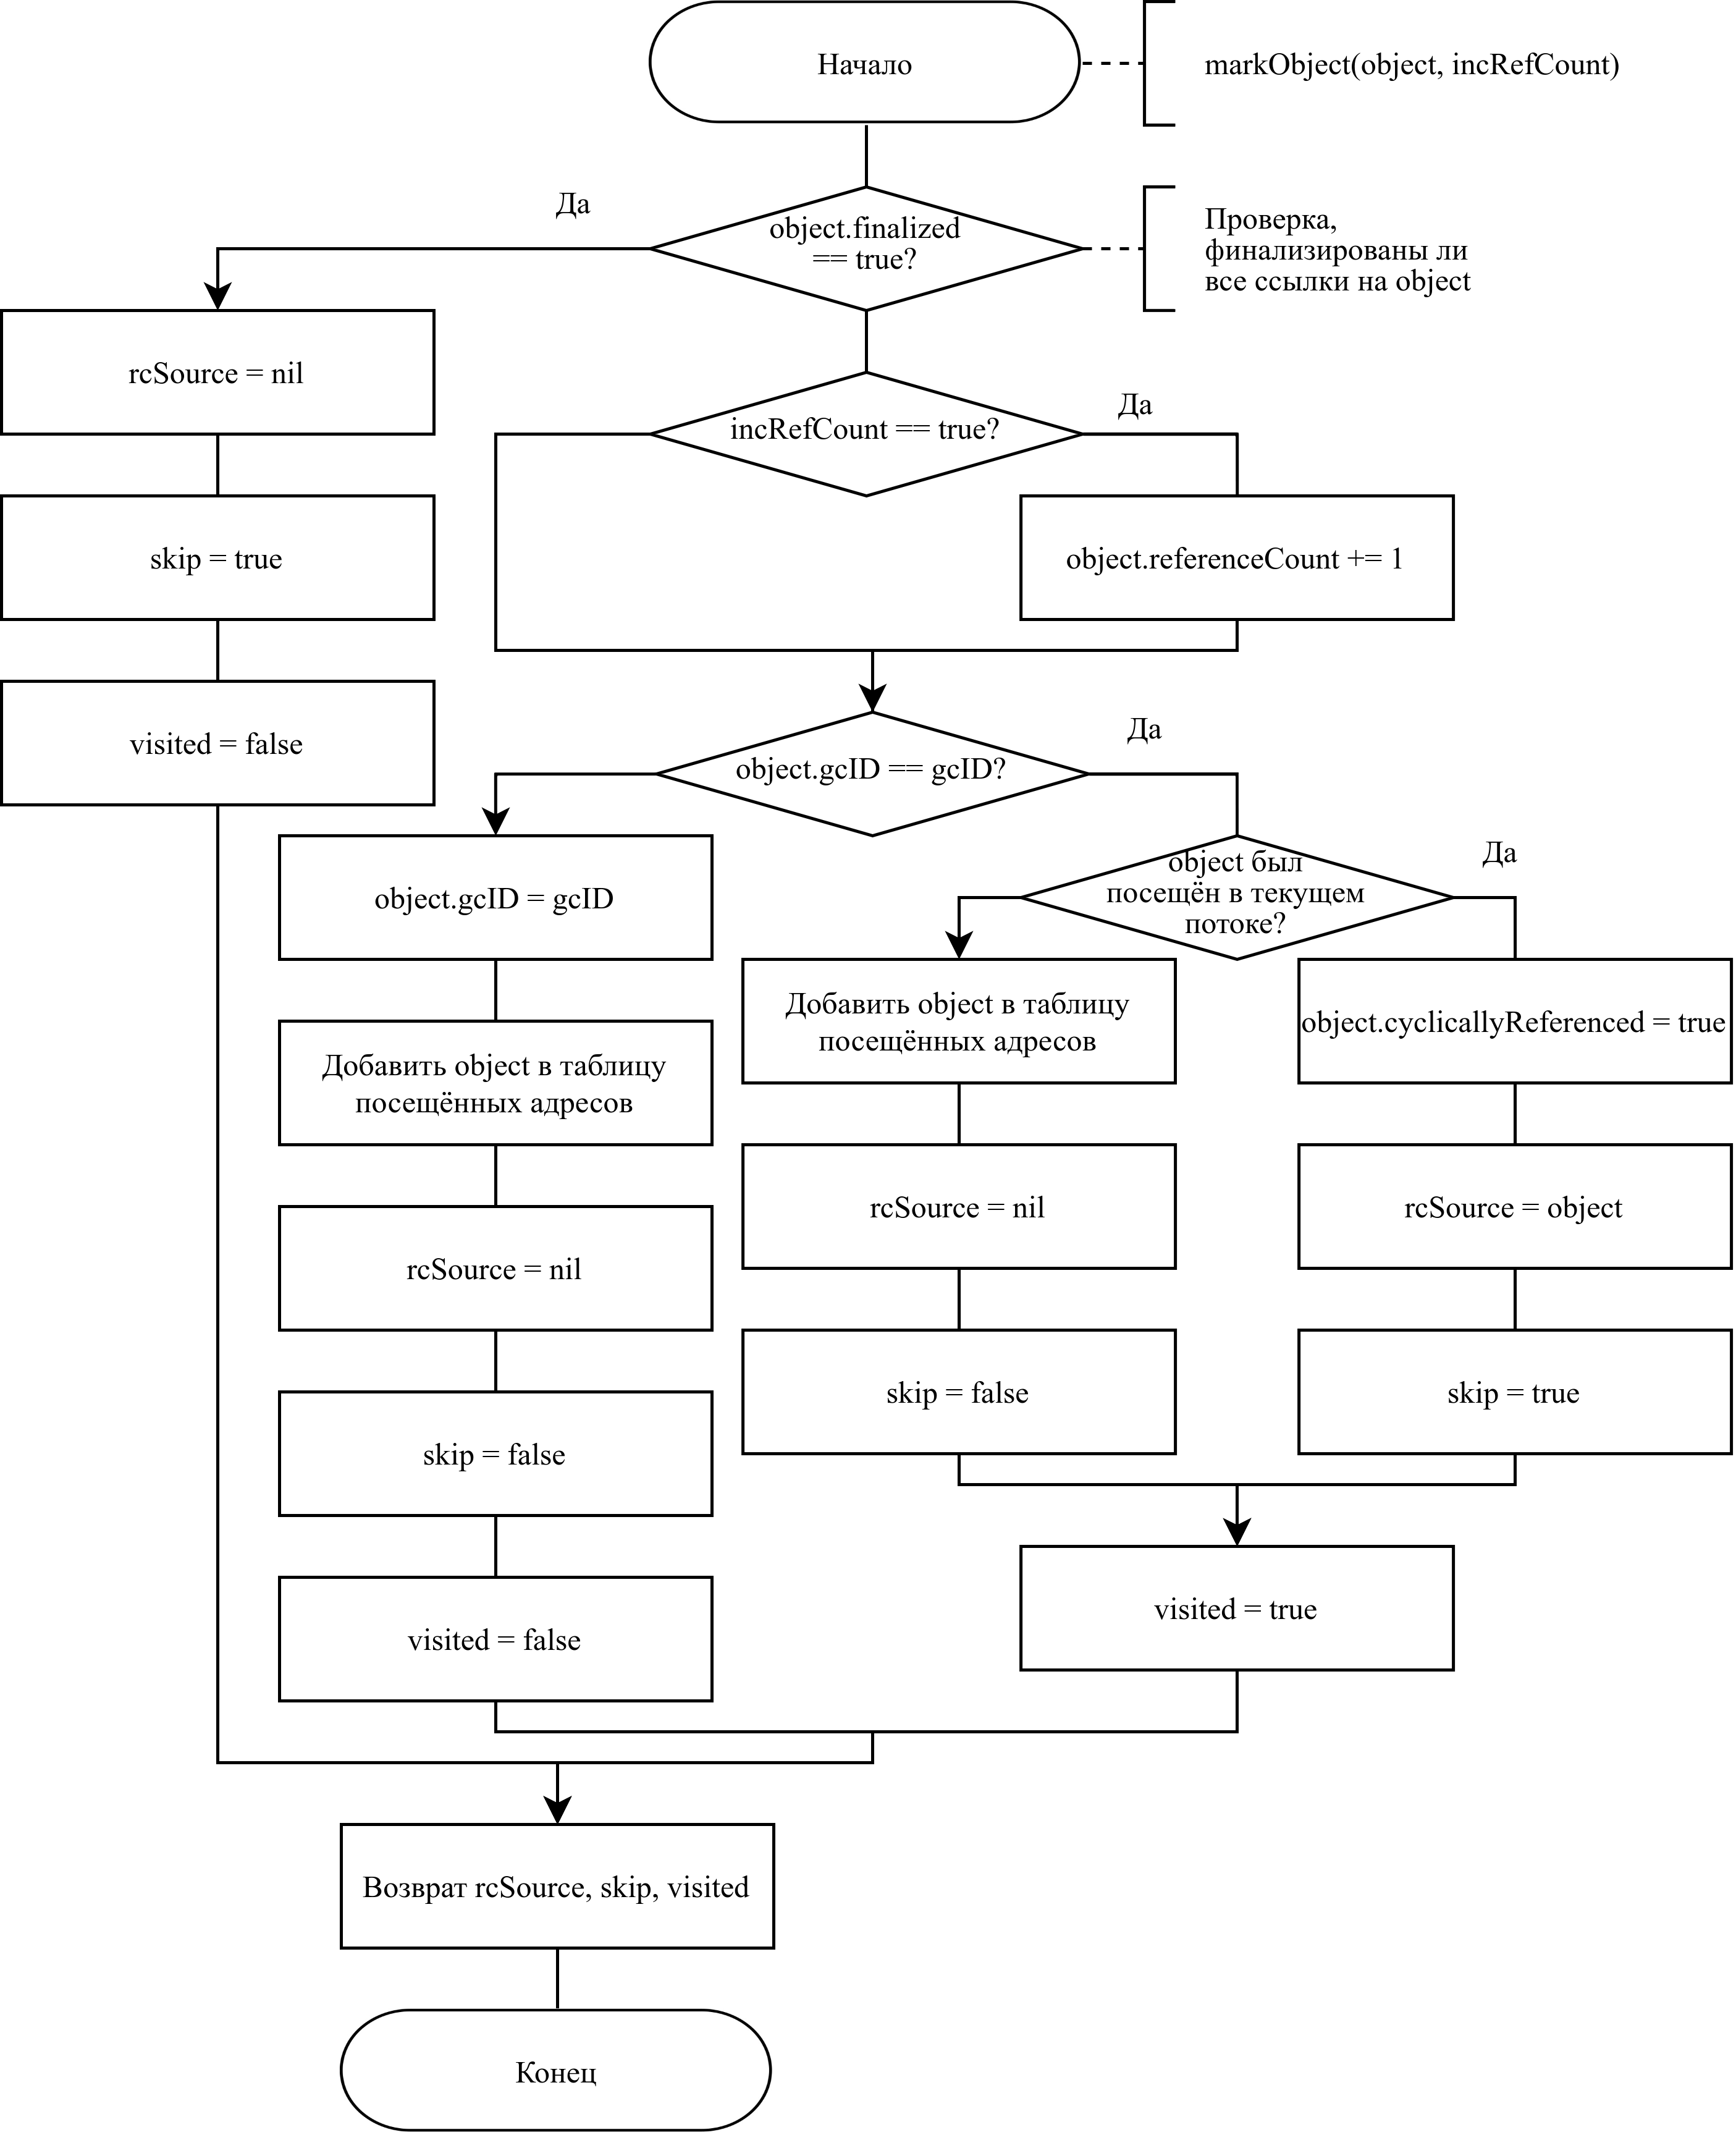
\includegraphics[scale=0.185]{assets/mark-4.png}
	\caption{Алгоритм анализа ссылок объекта}
	\label{fig:mark-4}
\end{figure}

\subsubsection{Очистка}

На рисунке \ref{fig:sweep-1} представлен алгоритм очистки поколения от мусорных объектов. Для дальнейшего принятия решения о перераспределении объектов между поколениями, рассматриваемый алгоритм подсчитывает размер поколения до и после очистки. В данном контексте размер измеряется в аренах.

\begin{figure}[H]
	\centering
	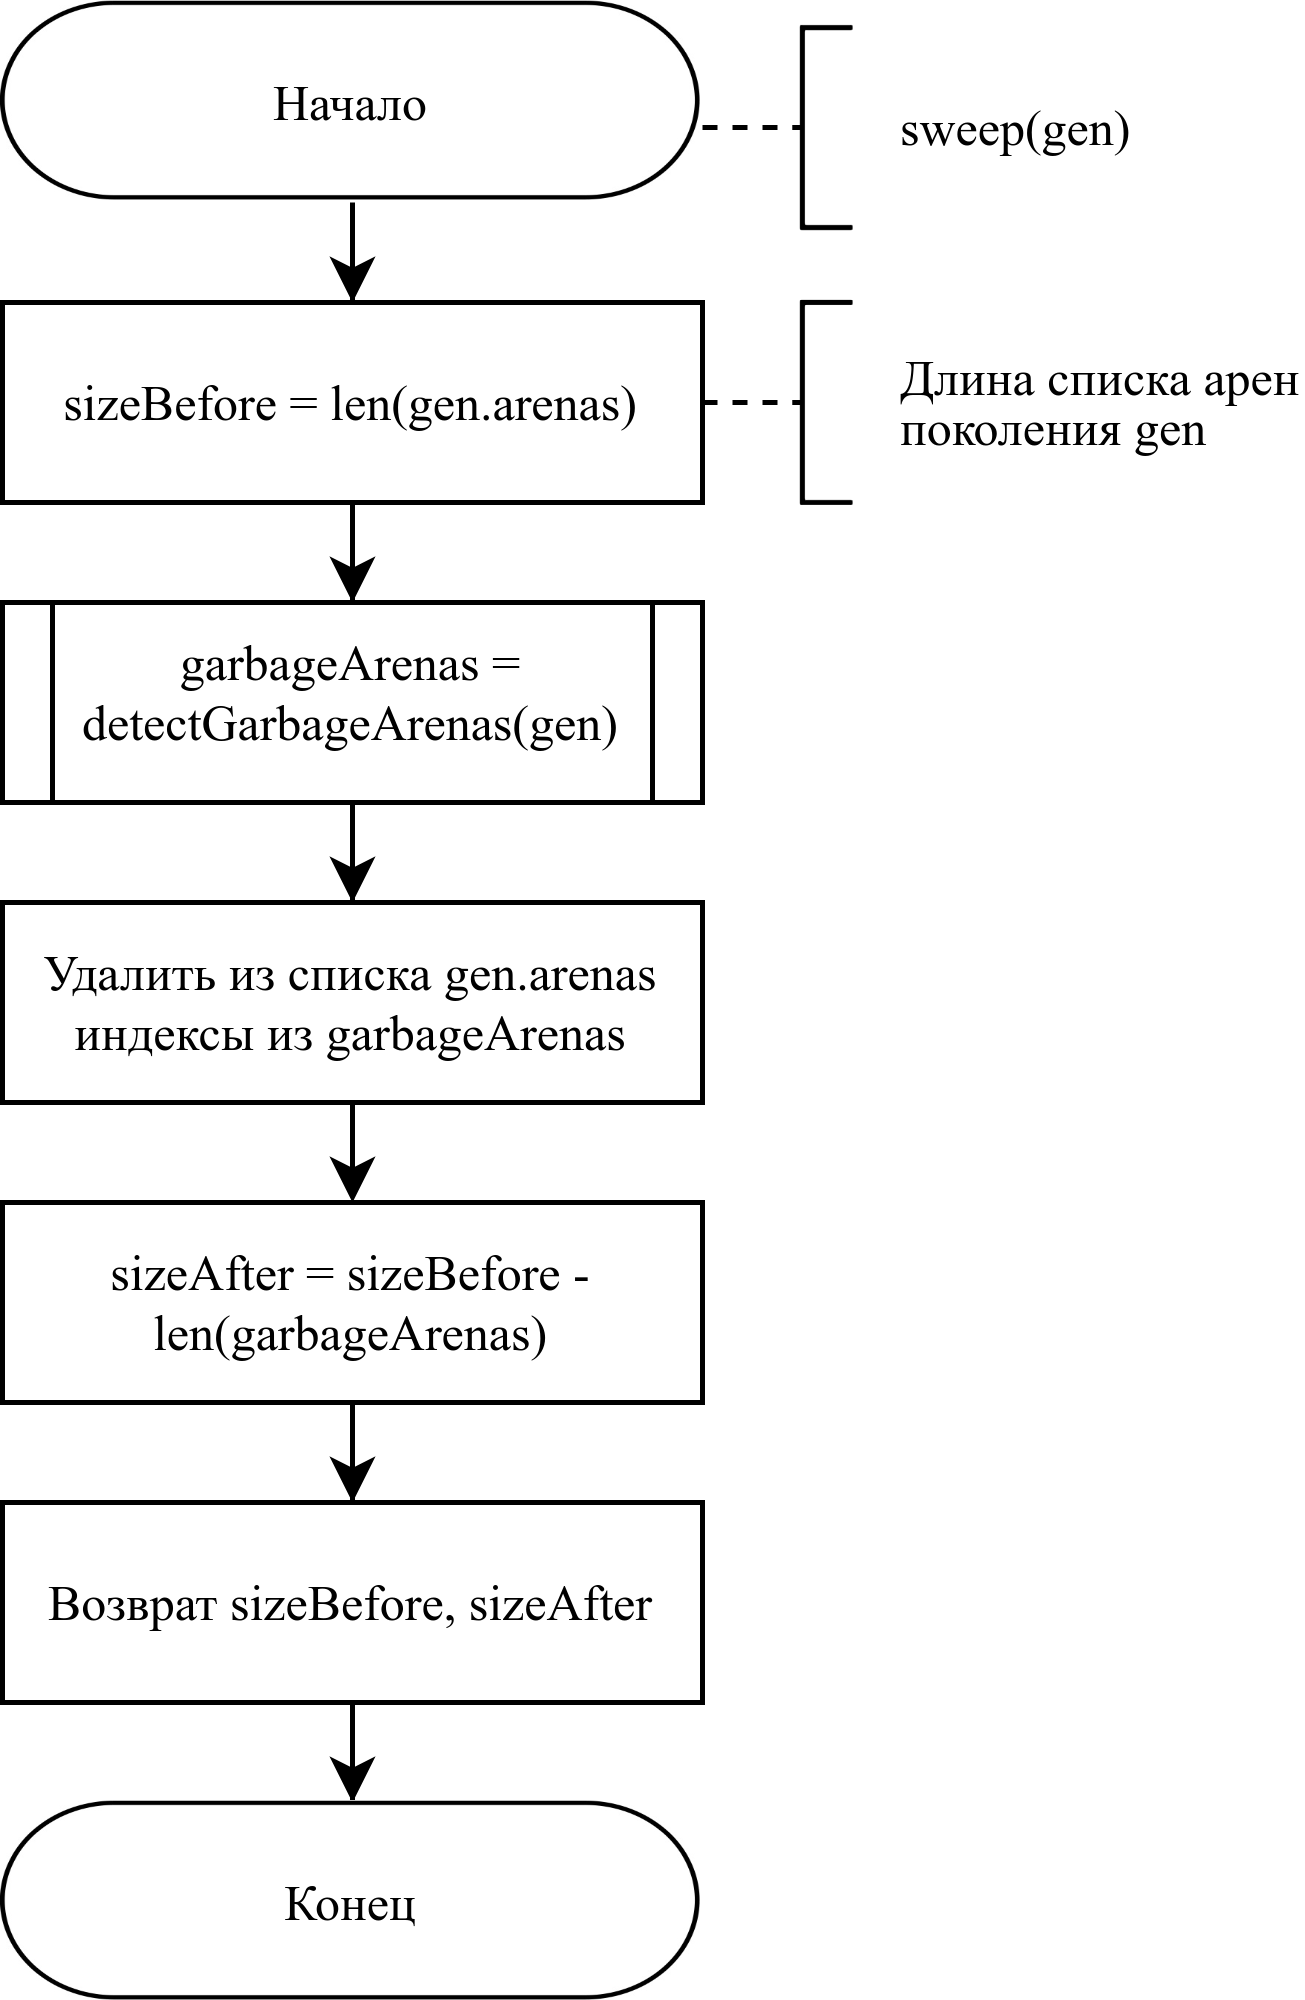
\includegraphics[scale=0.185]{assets/sweep-1.png}
	\caption{Алгоритм очистки поколения от мусорных объектов}
	\label{fig:sweep-1}
\end{figure}

На рисунках \ref{fig:sweep-2} и \ref{fig:sweep-3} представлен алгоритм обнаружения мусорных арен для их последующего освобождения. Арена считается мусорной, если все объекты, которые в ней были выделены на момент анализа, являются мусором. Такое определение мусорной арены может приводить к ситуациям, когда арена не может быть освобождена из-за наличия в ней живых объектов, суммарный размер которых много меньше размера арены. Данная проблема решается по-разному в зависимости от средств реализации, но в общем случае можно предложить выбор оптимального размера арены памяти, при котором частота возникновения описанных ситуаций пренебрежимо мала.

\begin{figure}[H]
	\centering
	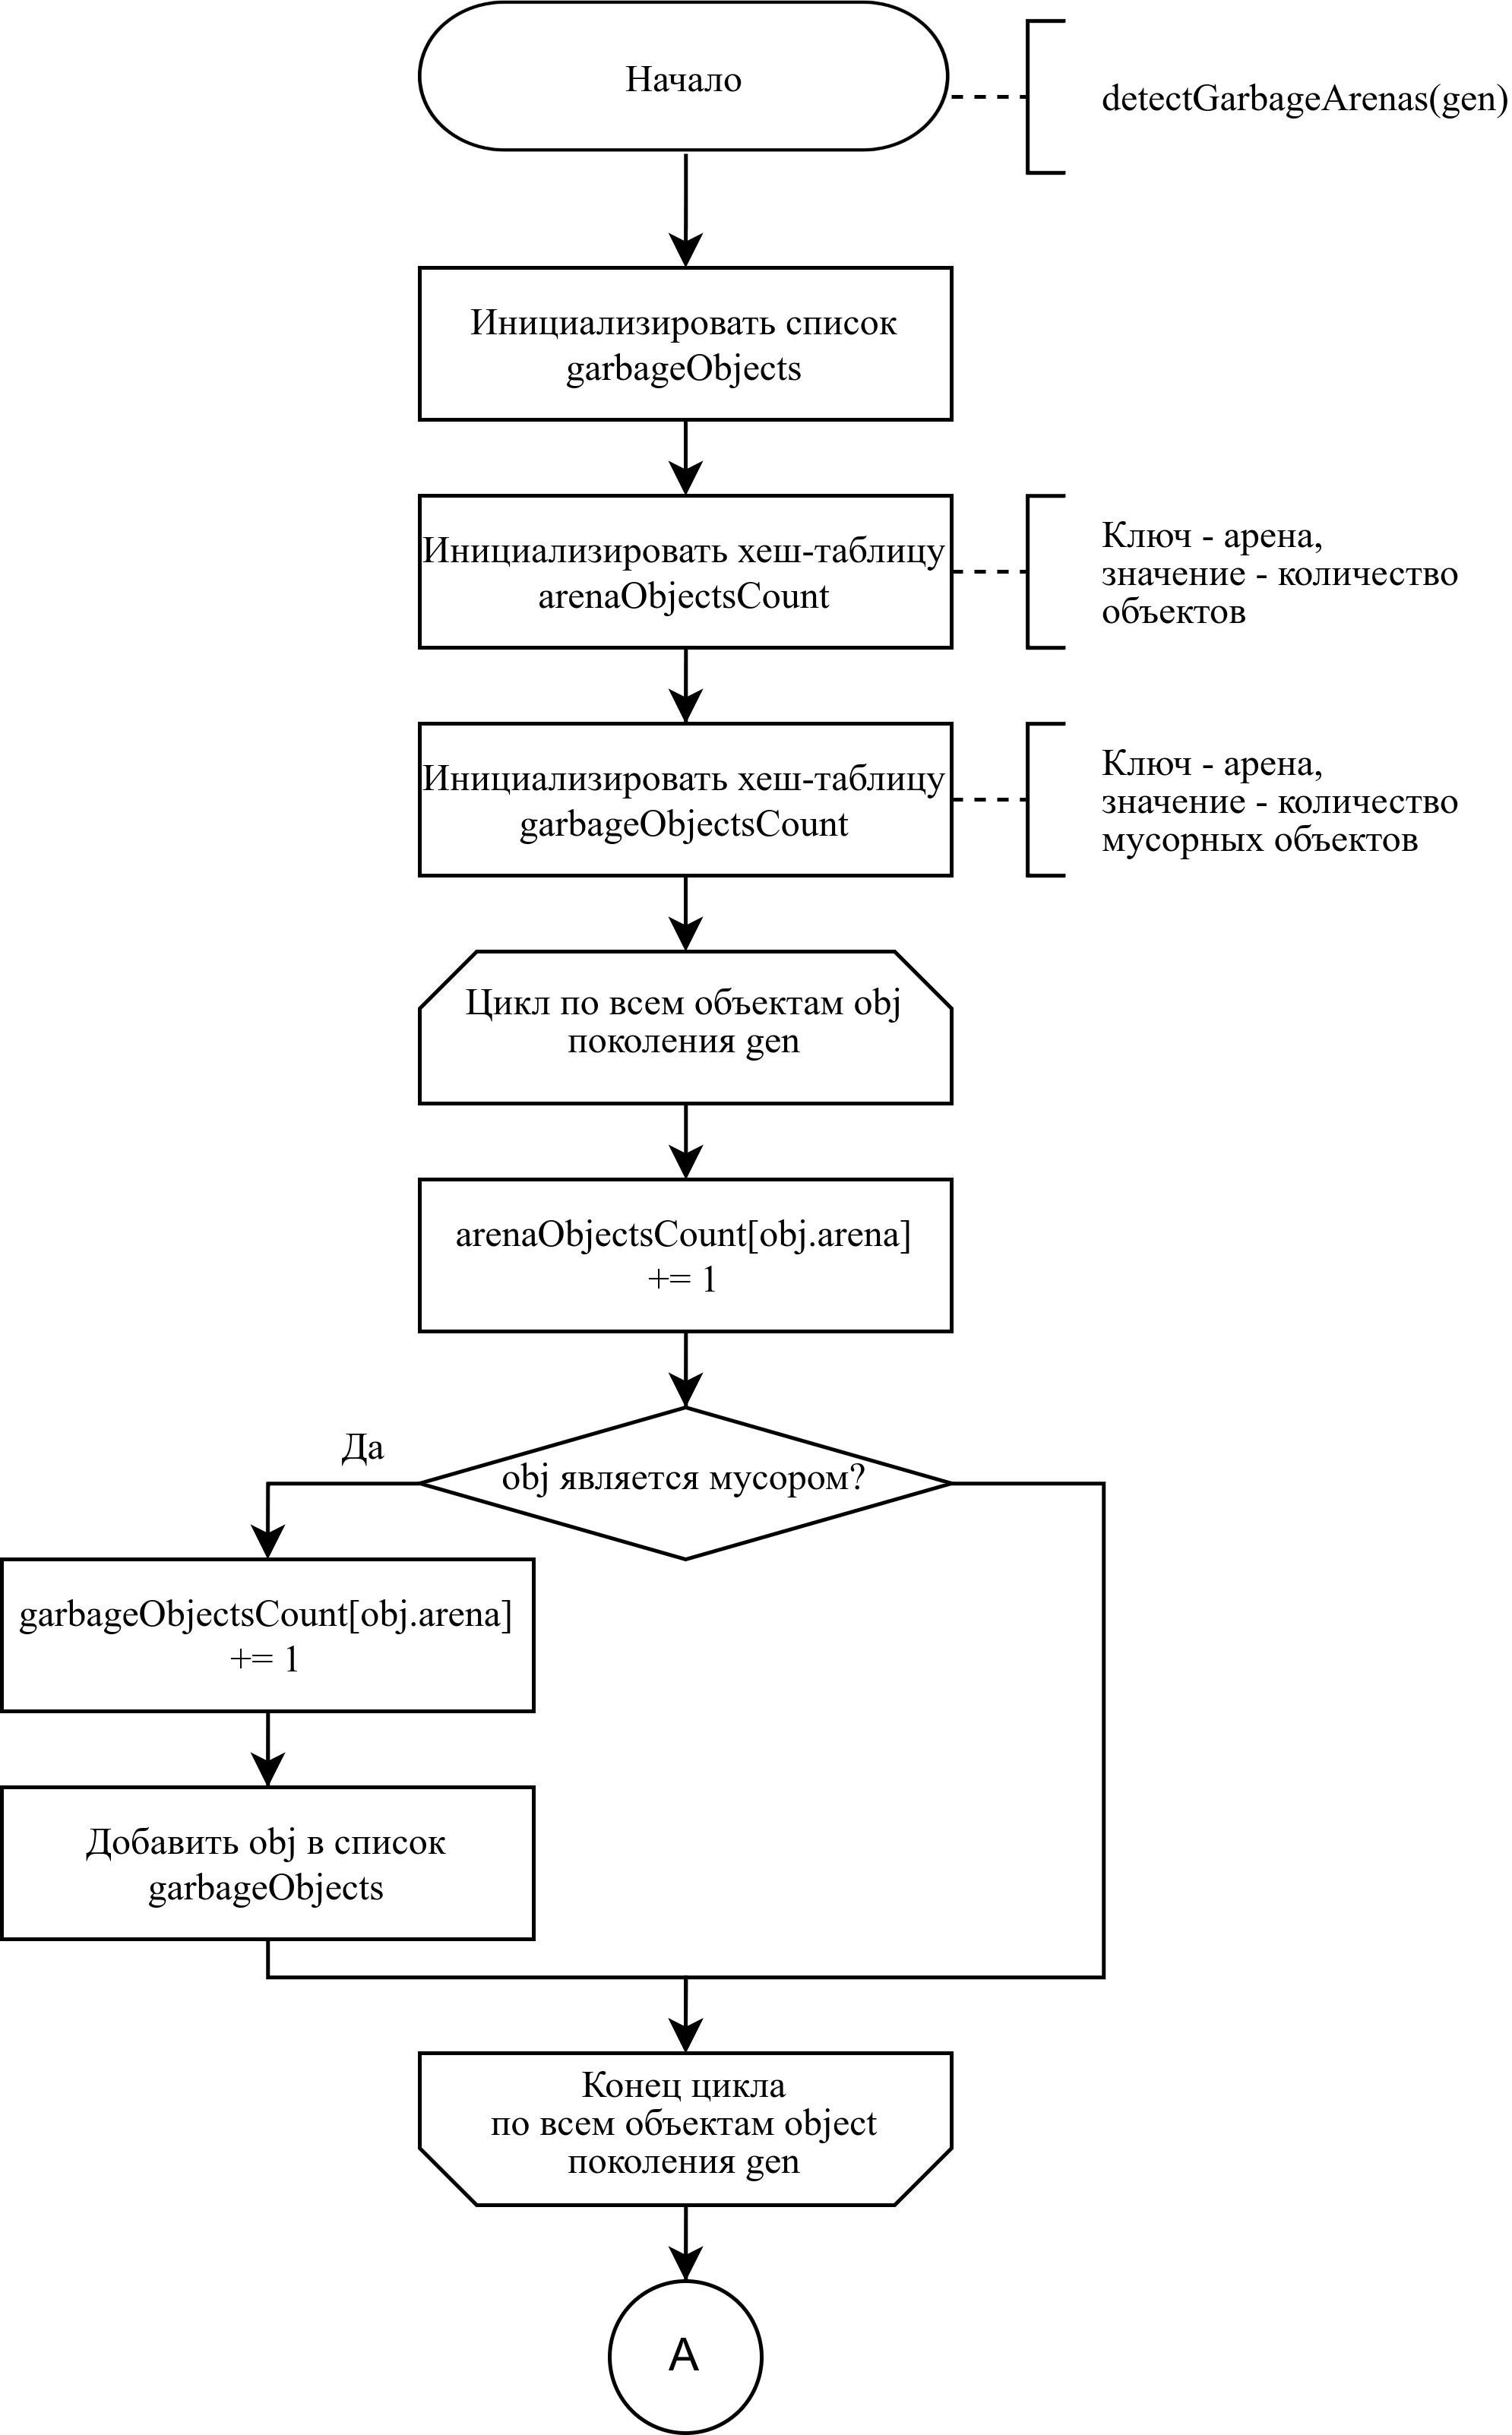
\includegraphics[scale=0.185]{assets/sweep-2.png}
	\caption{Алгоритм обнаружения мусорных арен, часть 1 (подсчёт дескрипторов объектов)}
	\label{fig:sweep-2}
\end{figure}

\begin{figure}[H]
	\centering
	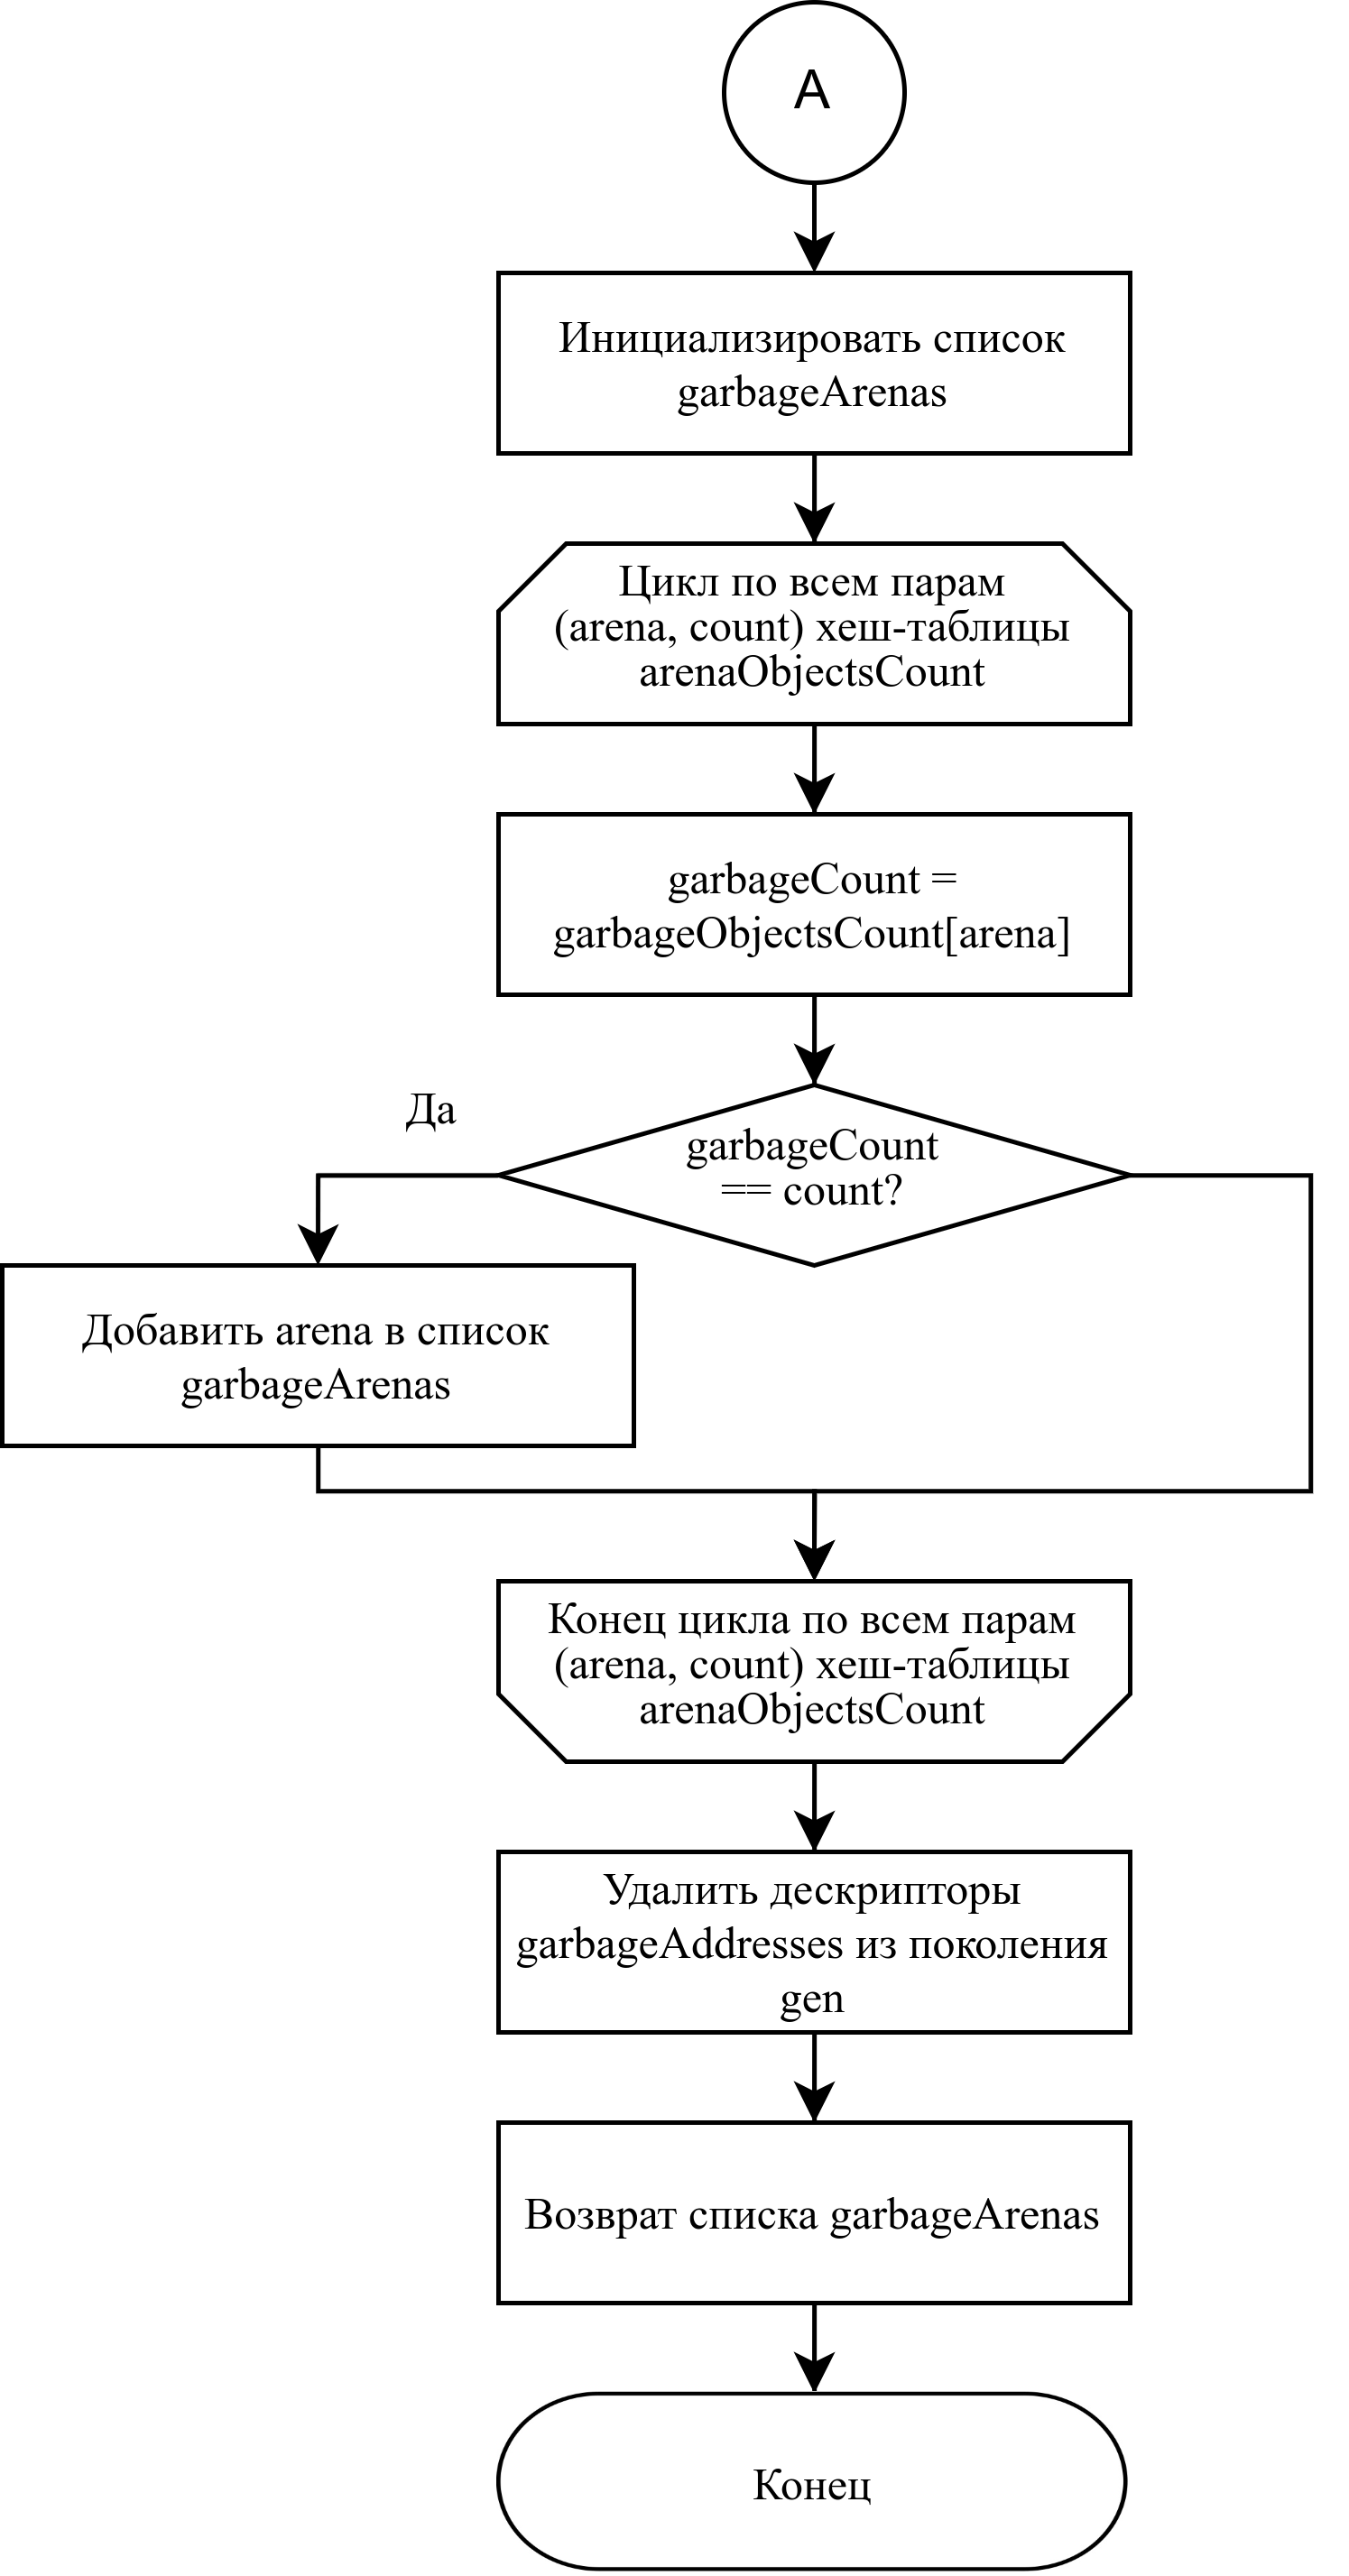
\includegraphics[scale=0.185]{assets/sweep-3.png}
	\caption{Алгоритм обнаружения мусорных арен, часть 2 (формирование результата и очистка мусорных дескрипторов)}
	\label{fig:sweep-3}
\end{figure}

\subsubsection{Перераспределение объектов между поколениями}

На рисунке \ref{fig:relocate} представлен алгоритм перераспределения объектов между поколениями. Порог перемещения поколения нужен для ограничения скорости продвижения объектов по поколениям.

\begin{figure}[H]
	\centering
	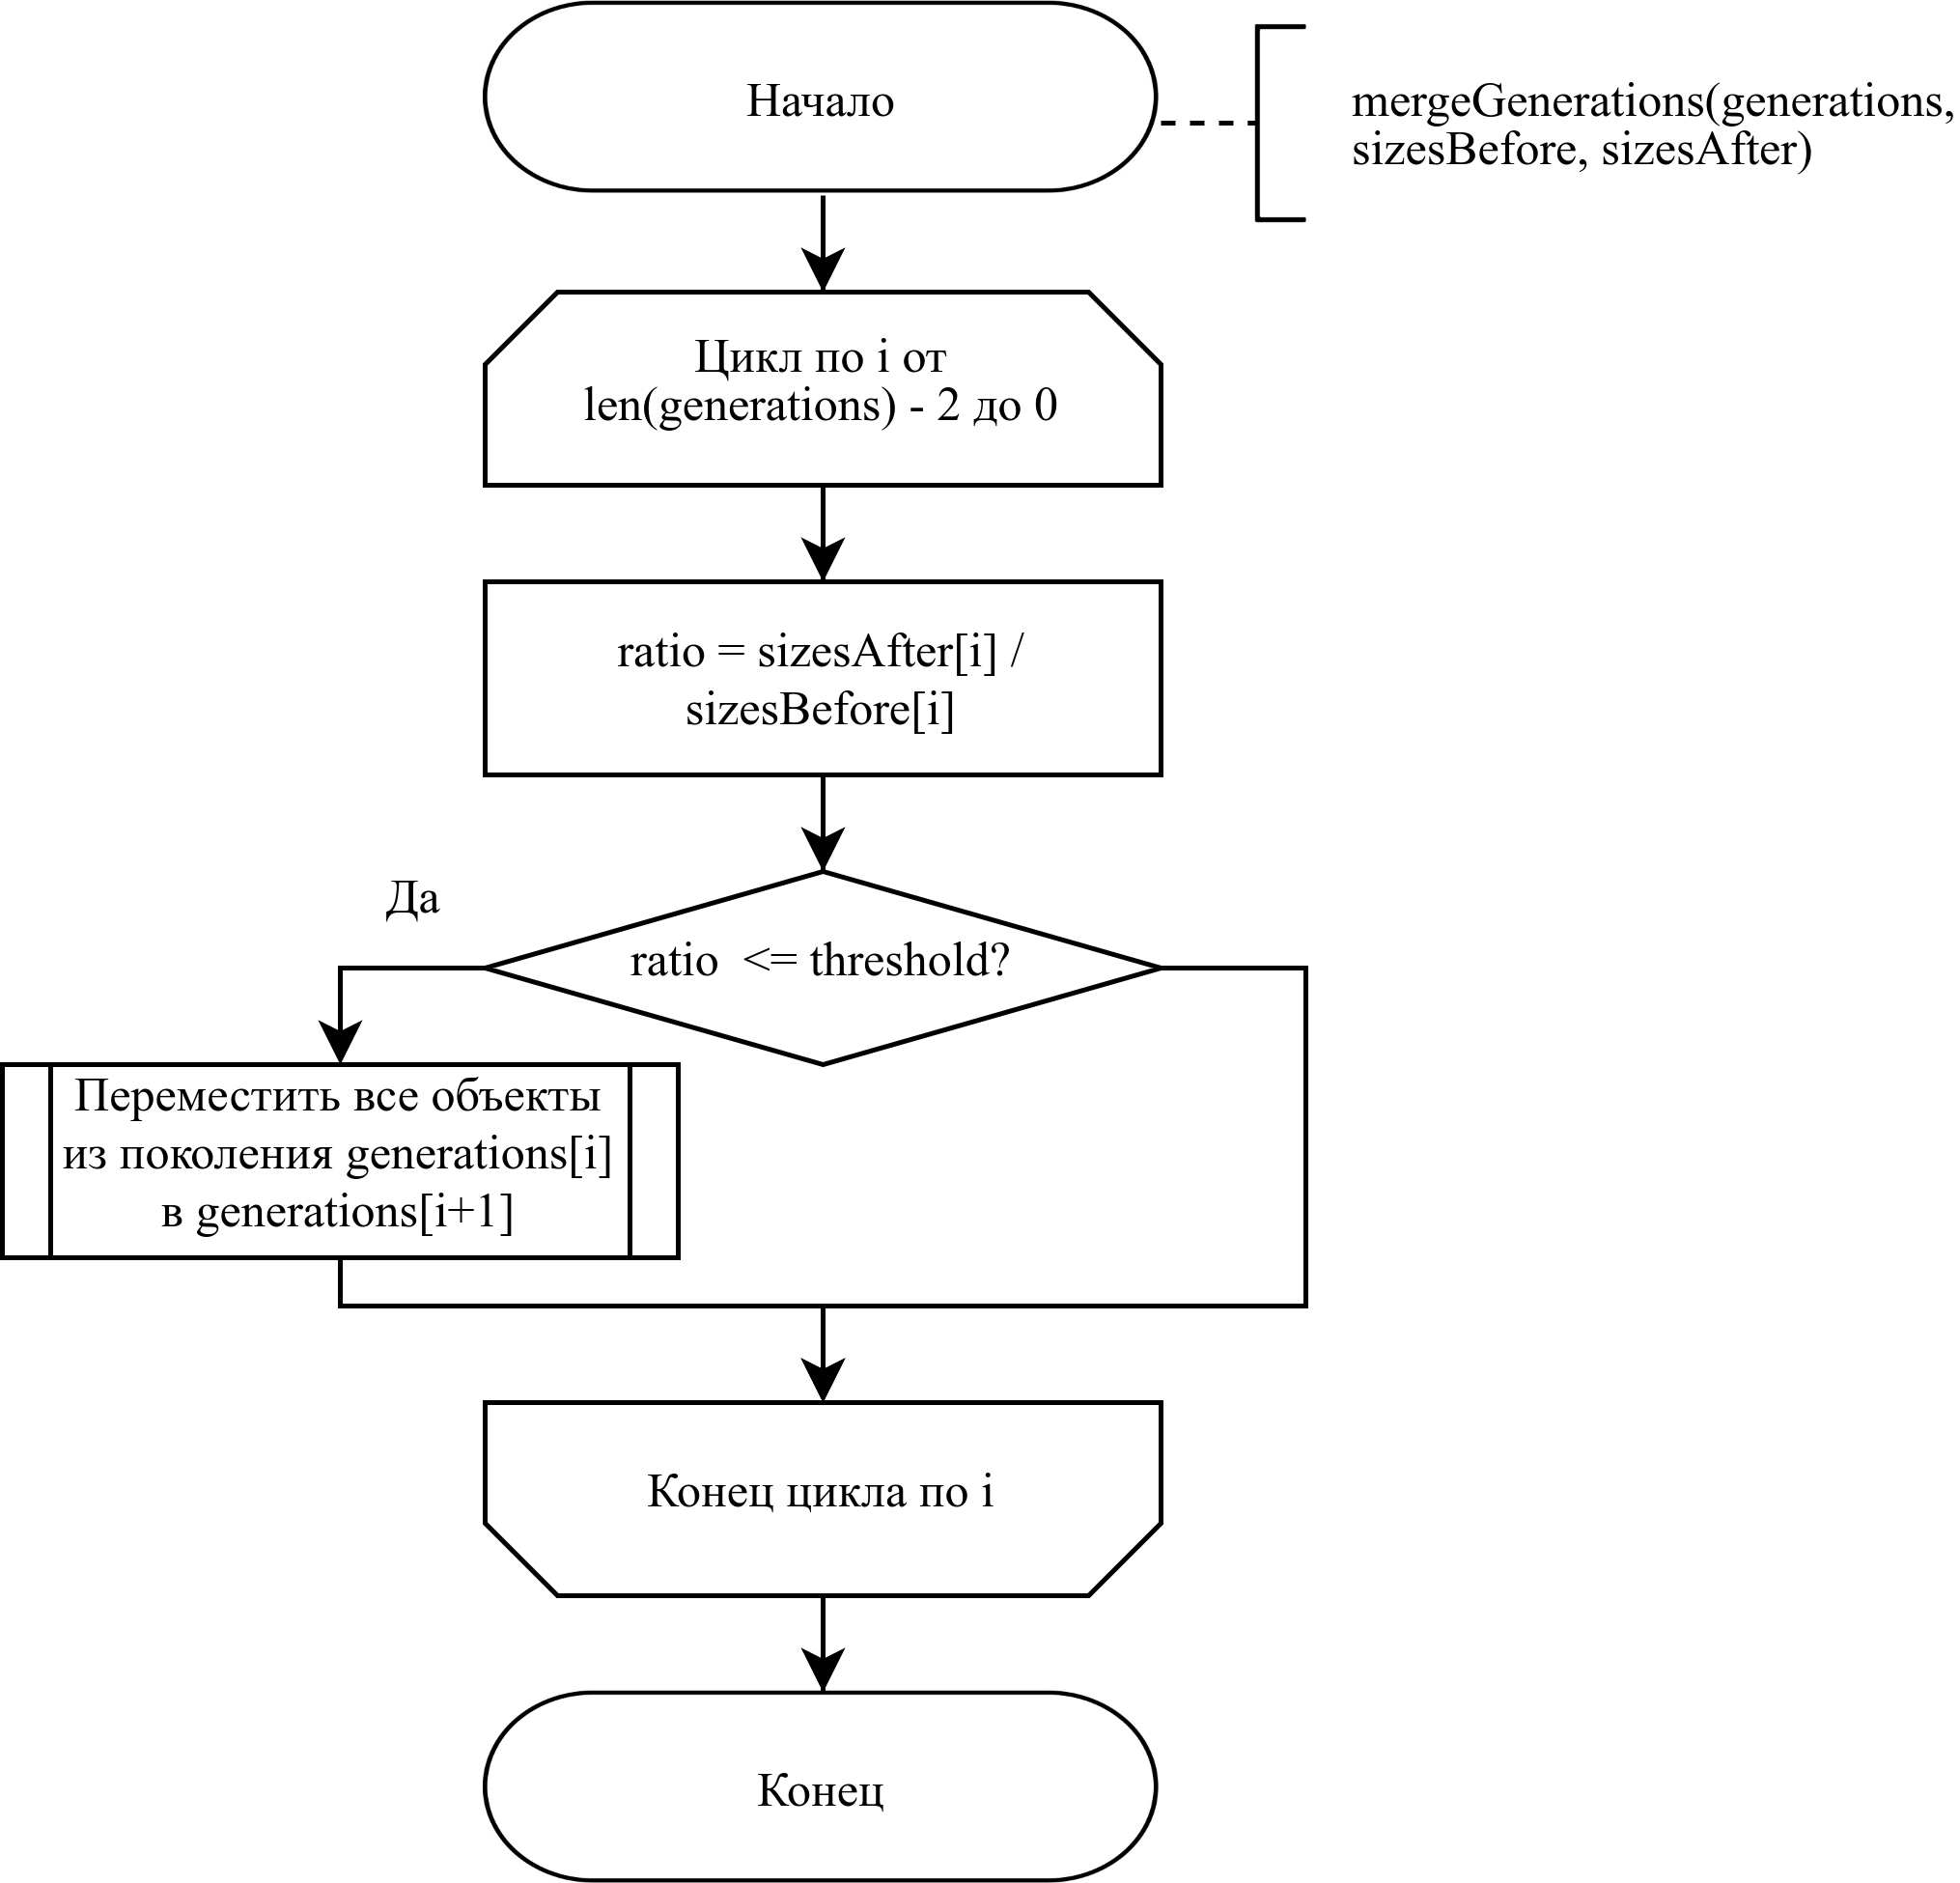
\includegraphics[scale=0.185]{assets/relocate.png}
	\caption{Алгоритм перераспределения объектов между поколениями}
	\label{fig:relocate}
\end{figure}




\section{Выбор структуры данных для хранения дескрипторов объектов}

Алгоритмы выделения памяти и сборки мусора предполагают наличие контейнера дескрипторов объектов. Основываясь на особенностях разработанных алгоритмов, можно сделать вывод о том, что операция поиска элемента будет выполняться гораздо чаще, чем операции вставки и удаления. Следовательно, главным критерием выбора структуры данных для хранения дескрипторов объектов будет являться временная трудоёмкость выполнения операции поиска.

Среди различных типов структур данных самыми эффективными с точки зрения поиска элементов являются
\begin{itemize}[label*=---]
	\item хеш-таблицы (сложность поиска $O(1)$ в лучшем случае, $O(N)$ в худшем);
	\item деревья ($O(log N)$ в лучшем и худшем случае, если рассматривать, например, красно-чёрные деревья);
	\item отсортированные массивы ($O(log N)$ в лучшем и худшем случае при использовании алгоритма бинарного поиска).
\end{itemize}
Все перечисленные структуры данных требуют затрат памяти, линейно зависящих от количества элементов.

Отсортированный массив не подходит для хранения дескрипторов объектов, поскольку хранит данные в памяти последовательно, и с увеличением количества объектов затраты времени и памяти на перевыделение массива будут расти, приводя к задержкам мутатора при выделении новых объектов.

Между хеш-таблицами и деревьями рекомендуется выбрать хеш-таблицу по причине меньшей временной сложности поиска элемента в лучшем случае. Доля случаев, в которых сложность поиска элемента в хеш-таблице составляет не $O(1)$, а $O(1)-O(N)$, зависит от выбора хеш-функции для ключей.

Стоит отметить, что оптимальность выбора структуры данных для хранения дескрипторов объектов может зависеть от особенностей языка реализации.

\section{Выбор подхода к реализации метода}

Разработанные алгоритмы распределения памяти можно реализовать одним из следующих способов.

\begin{enumerate}[label*=\arabic*.]
	\item В виде модификации компилятора или интерпретатора языка. Такой подход предоставляет больше возможностей для использования собственных барьеров чтения и записи объектов, позволяет безопасно выполнять копирование или перемещение отдельно взятых объектов программы, а также напрямую влиять на работу основного сборщика мусора, если его наличие предусмотрено языком реализации метода. % + для сравнения методов не обязательно менять исходный код приложения?
	\item В виде подключаемой библиотеки. Данный способ позволяет не зависеть от метода распределения памяти, предусмотренного языком реализации метода, а также имеет больше применим на практике, поскольку добавление новой библиотеки в пользовательский проект является более гибким подходом, чем настройка в проекте работы с другим компилятором или интерпретатором, поскольку позволяет выбирать методы распределения памяти для каждого модуля приложения, а также сравнивать их при использовании в одном отдельно взятом модуле.
\end{enumerate}

Оба описанных подхода к реализации предполагают добавление новой зависимости в пользовательских проектах. Описанные ранее алгоритмы работы менеджера памяти спроектированы таким образом, чтобы их выполнение можно было совмещать с работой сборщика мусора, встроенного в язык программирования реализации. При этом не требуется напрямую влиять на его работу, а также иметь возможность копировать и перемещать объекты, так как сборщики мусора, работающие по алгоритму mark-sweep являются неперемещающими. Следовательно, вариант реализации метода в виде подключаемой бибилотеки является наиболее предпочтительным ввиду большей практической применимости.

%Обосновать в конструкторском разделе выбор между реализацией в виде модификации компилятора (можно вставлять кастомные барьеры чтения и записи (реализовываать их нативно), выполнять копирование и перемещение объектов, влиять на процесс разметки кучи  и т.д.) и в виде подключаемой библиотеки: 
%- нет лишней мишуры => работает быстрее
%(ЦЕЛЬ ДИЗАЙНА РАЗРАБАТЫВАЕМОГО МЕНЕДЖЕРА ПАМЯТИ - МАКСИМАЛЬНО БЫСТРОЕ ВЫДЕЛЕНИЕ без лишней нагрузки на мутаторы)
%- полностью заменить стандартный менеджер памяти своими патчами на компилятор нельзя, так как многие популярные библиотеки зависят от него => надо как-то уживаться с GC
%- применимость на практике: подключить либу легче и удобнее, чем качать другой компилятор (по сути новый язык)

%Нельзя безопасно обновлять указатели (?????), поэтому копировать объекты нельзя
%+ Меньше накладных расходов
%- Беды с фрагментацией




\section*{Выводы из конструкторской части}

В данном разделе были разработаны алгоритмы основные этапов метода автоматического управления памятью с гарантированным временем выполнения на основе подсчёта ссылок. Был описан подход к реализации метода.	

Исходя из количества данных, которые хранит в себе дескриптор объекта, можно выдвинуть предположение о том, что метод будет иметь наибольшую эффективность при его использовании для аллокации объектов программы, которые не содержат циклических ссылок и занимают объём памяти, намного превышающий размер дескриптора объекта. Тогда накладные расходы на хранение дескрипторов объектов и сборку циклических ссылок будут пренебрежимо малы по сравнению с ресурсными затратами основной программы.


